\documentclass[twocolumn, 9pt]{jsproceedings}
\RequirePackage[l2tabu, orthodox]{nag}  % 古いコマンドやパッケージを使用した場合に警告する
\usepackage[all, warning]{onlyamsmath}  % amsmath が提供しない数式環境を使用した場合に警告する
% \usepackage{flushend}  % 最終ページの2カラムの左右の高さを揃える



\usepackage{otf}
\usepackage[ipa]{pxchfon}
\usepackage{caption}
\usepackage{graphicx}

% タイトル
\title{つくばチャレンジ 2023 における\\千葉工業大学未来ロボティクス学科 box2,box3チームの取り組み}

\author{○今井 悠月,井口 颯人,樋高 聖人,春山 健太,藤原 柾,\CID{8705}橋 祐樹,白須 和暉,野村 駿斗,
望月 悠矢,\\馬場 琉生,村林 孝太郎,桜井 真希,中村 雄一,長島 昂生,\\上田 隆一,林原 靖男(千葉工大)}

\etitle{The activities of the Advanced Robotics Department box2 and box3 team of Chiba Institute of Technology in the Tsukuba Challenge 2023}

\eauthor{Yuzuki IMAI, Hayato IGUCHI, Masato HIDAKA, Kenta HARUYAMA, Masaki FUJIWARA, \\Yuki TAKAHASHI,
 Kazuki SHIRASU, Hayato NOMURA, Yuya MOCHIZUKI, Ryusei BABA, \\Koutarou MURABAYASHI, Maki SAKURAI,
 Yuichi NAKAMURA, Kousei NAGASHIMA, \\Ryuichi UEDA and Yasuo HAYASHIBARA (CIT)}

\affiliation{千葉工業大学未来ロボティクス学科 box2, box3チーム}

\abstract{
  In this paper, we present the activities of the Advanced Robotics Department box2 and box3 team of 
  Chiba Institute of Technology in the Tsukuba Challenge 2023. 
  We developed autonomous outdoor mobile robots, and we tackled several challenges. 
  For example, We developed robots using machine learning and robots that can run in the rain.
}


\begin{document}
\maketitle

% 本文
\section{緒言}
我々は,屋外でも正確に自律移動可能なロボットを目指し,その研究および開発の一環として
つくばチャレンジに参加している.
これまで本研究室\footnote{千葉工業大学未来ロボティクス学科 林原研究室}では,地図生成や自己位置推定を
中心に研究開発を行ってきた.近年では,防水機能や高い拡張性を有したオープンプラットフォームのロボットの
開発も行っている.
つくばチャレンジ2022では,開発したロボットやシステムを用いて,記録走行において完走を達成した.
しかし,本年度からは確認走行エリアのコースが一部変更され,つくば市役所の外周がコースに含まれるようになった.
そのため,30 m 程度の 2次元レーザレンジセンサ 1つでは,低層の茂みや障害物などを検出しつつ,
安定して自己位置推定を行うのが困難となった.
また,道幅の狭い経路を通る必要があるため,従来のシステムよりもロバストなシステムが要求された.
本稿では,このような問題を解決するためにつくばチャレンジ2023に向けて取り組んだ内容に関して紹介する.

\section{開発中のロボット}
ロボットを常に屋外環境で走行させるためには,防水設計が求められる.ただし,防水性を担保しながら
ロボットの機構や電気回路の追加および変更を行うことは,作業の負担が大きいと考えられる.
さらに,これらの作業には多くの時間を要するため,新たなアルゴリズムの開発や検証に十分な時間を割当てられない
ことが問題となっていた.

このような問題を踏まえ,本研究室では屋外自律移動ロボットプラットフォーム ORNE-boxの開発を行ってきた\cite{box}.
日々検証と改良を重ねており,現在は,3台のロボット(ORNE-box,ORNE-box2,ORNE-box3)がある.
これらのロボットは,屋外での自律走行を目的としており,屋外自律走行の研究開発に必要な機能をパッケージ化
し,提供することを目標に開発を行っている.設計データなどは,ウェブページ上にて順次公開している\cite{box-data}.

ORNE-box2 は,ORNE-box の問題点を洗い出し改善を図るという方針のもと,昨年度から開発を行っている.
センサ構成などに差異はあるが,基本的なシステム構成は同じである.

ORNE-box3 は,今年度から開発を行っており,ORNE-box2 の防水性能や拡張性をさらに強化した設計となっている.

\subsection{ハードウェア}
ORNE-box-Series の外観を\figref{fig:orne-series},仕様を\tableref{table:1}に示す.
これらのロボットは,i-Cart middle\cite{icart} をベースとしている.

\begin{figure}[h]
  \centering
  \begin{minipage}[b]{0.3\linewidth}
    \centering
    \includegraphics[width=21.1mm]{fig/box.pdf}
    \caption*{(a) ORNE-box}
  \end{minipage} 
  \hspace{-1.2mm}
  \begin{minipage}[b]{0.3\linewidth}
    \centering
    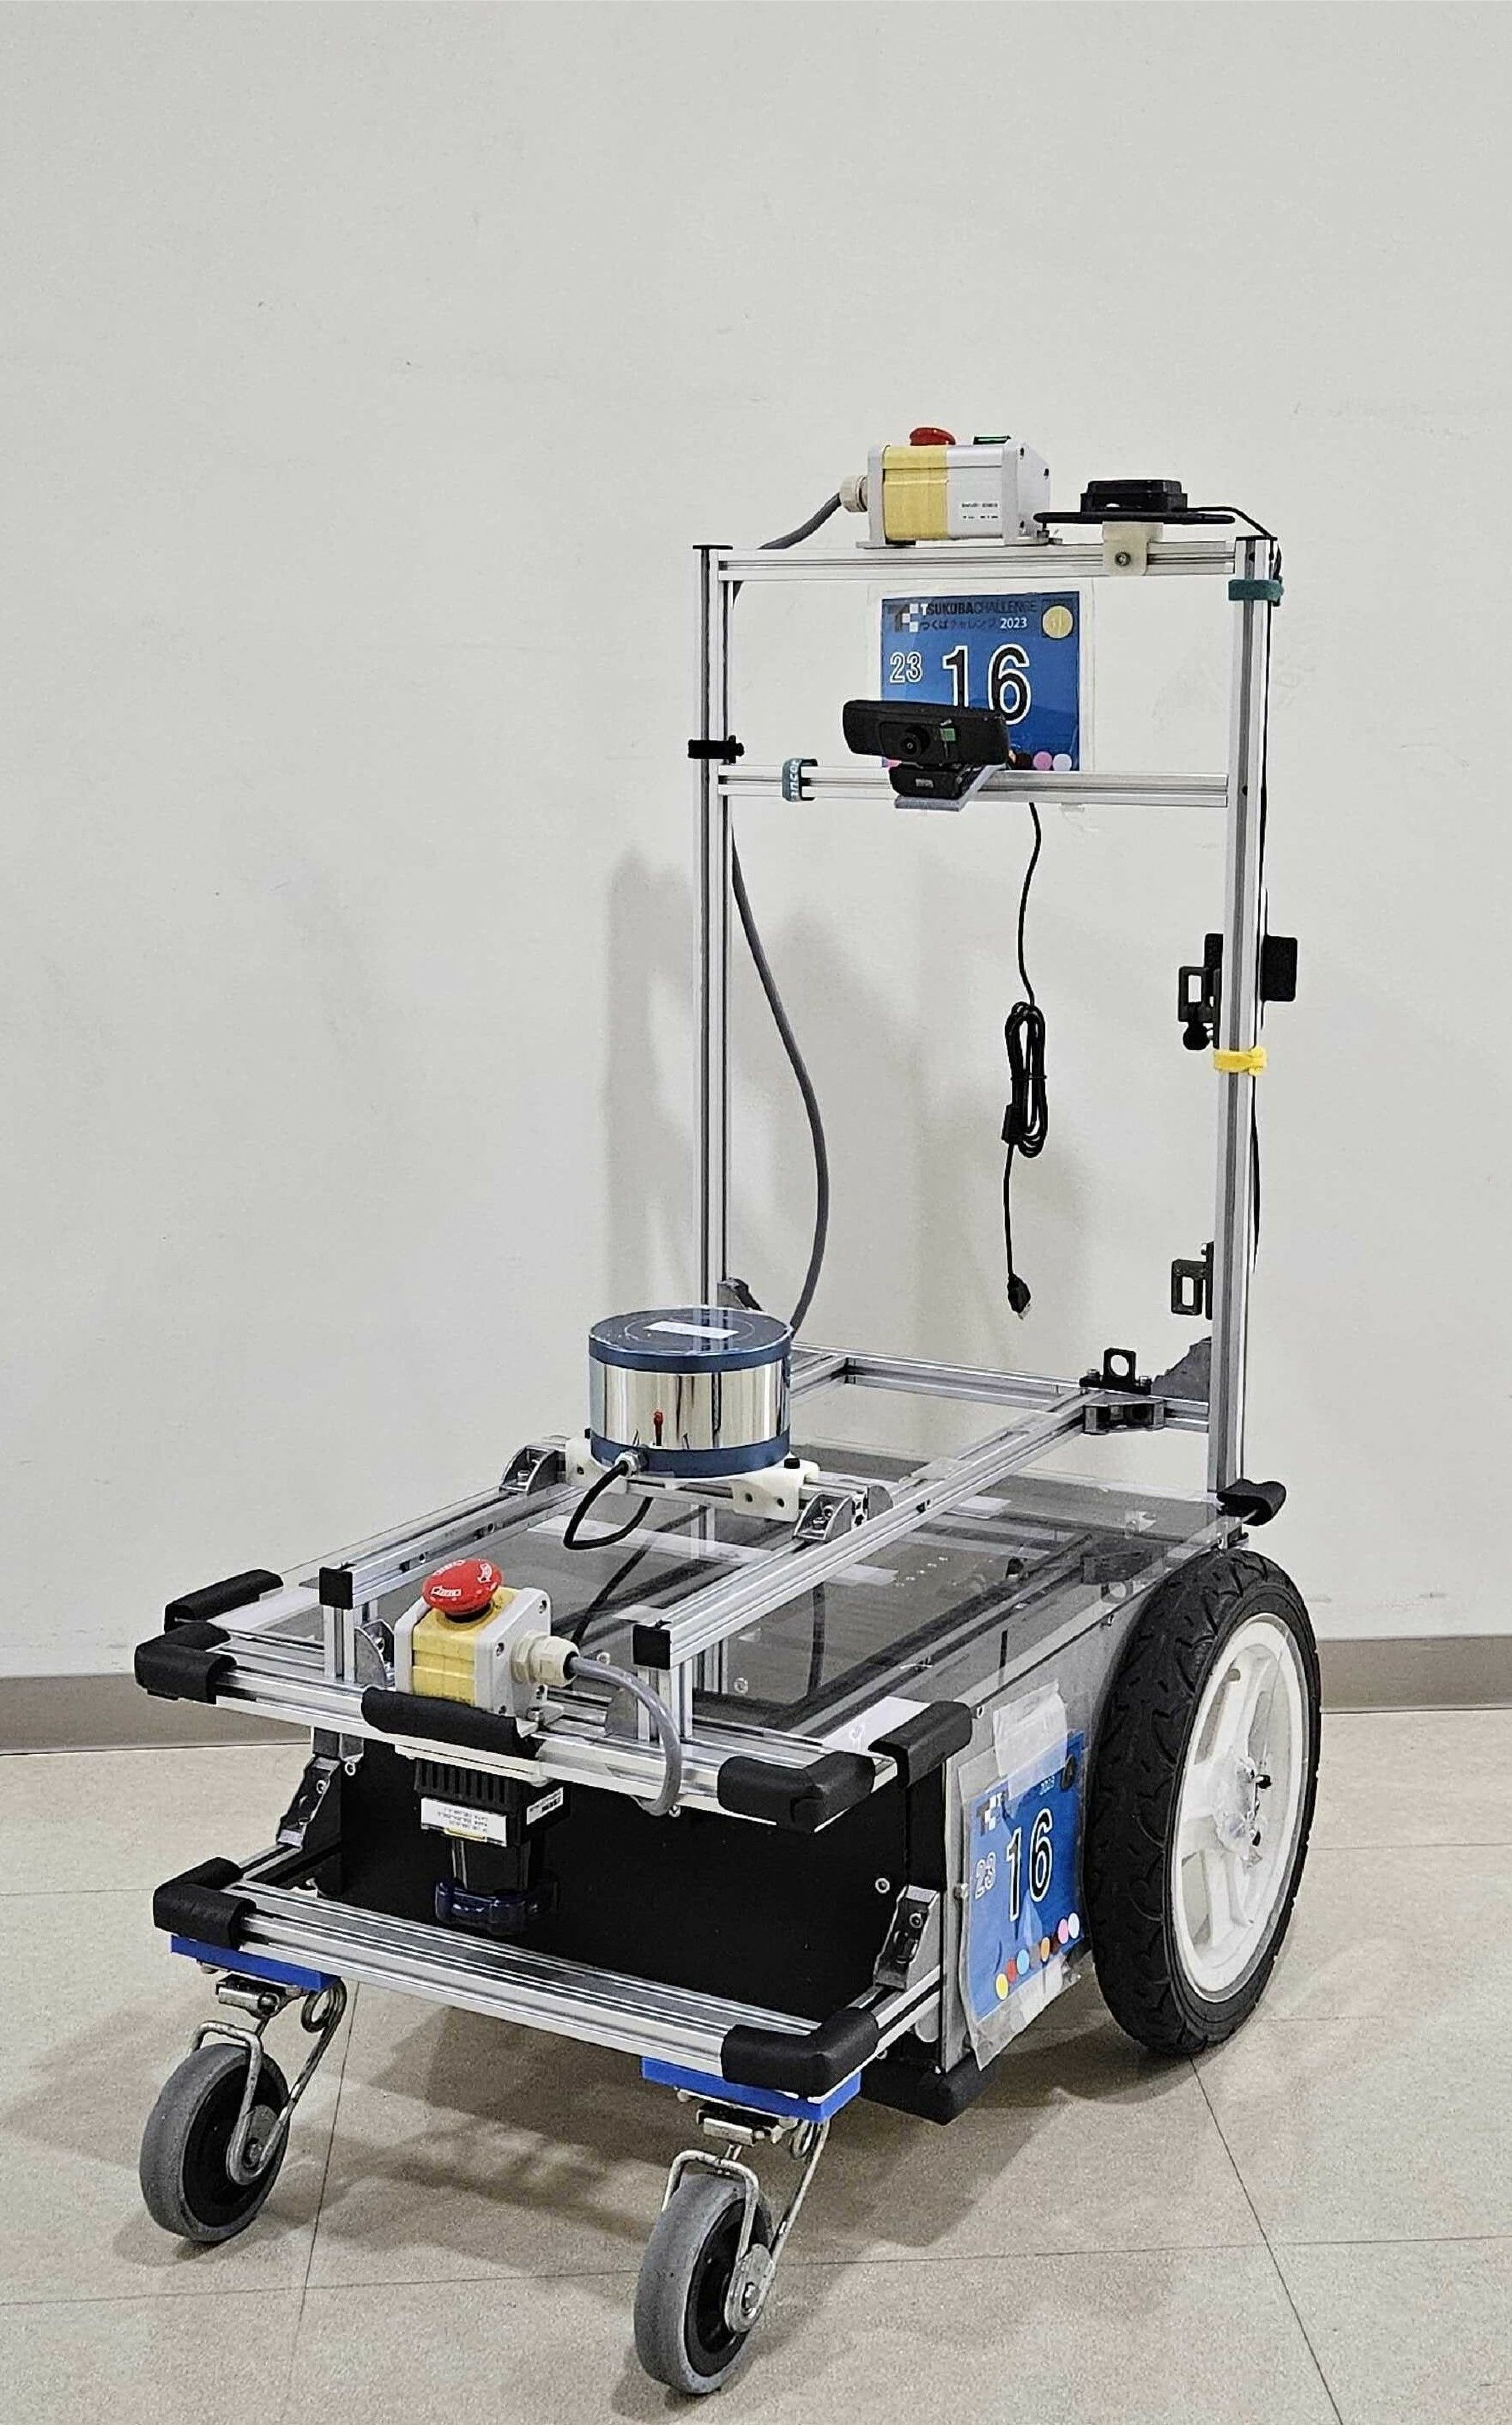
\includegraphics[height=34mm]{fig/box2.pdf}
    \caption*{(b) ORNE-box2}
  \end{minipage}
  \begin{minipage}[b]{0.3\linewidth}
    \centering
    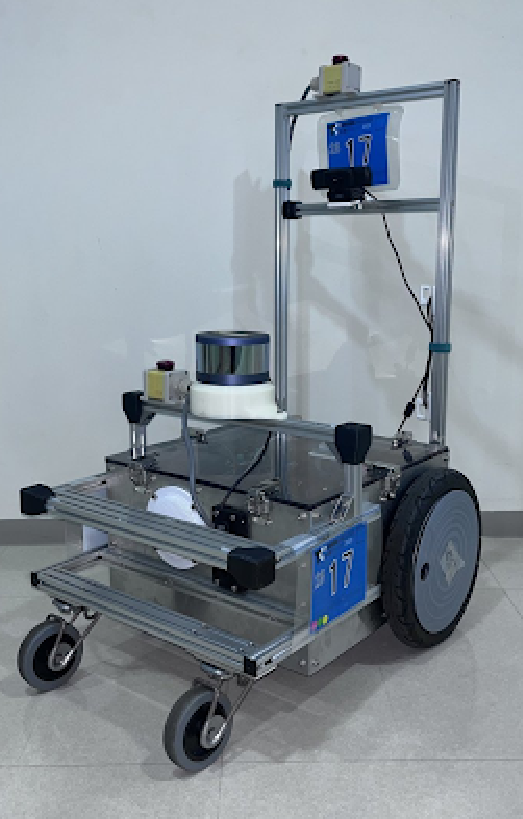
\includegraphics[height=34mm]{fig/box3.pdf}
    \caption*{(c) ORNE-box3}
  \end{minipage}
  \caption{ORNE-box-Series}
  \label{fig:orne-series}
\end{figure}

\vspace*{-4mm}

\begin{table}[h!]
  \centering
    \caption{Specifications of the robots.}
    \label{table:1}
    \scalebox{0.73}{
    \begin{tabular}{|l||c|c|c|}  \hline
      & ORNE-box & ORNE-box2 & ORNE-box3 \\ \hline \hline
      Depth[mm] & \multicolumn{2}{c|}{600} & ??? \\ \hline
      Wide[mm] & \multicolumn{2}{c|}{506.5} & ??? \\ \hline
      Height[mm] & \multicolumn{2}{c|}{957} & ??? \\ \hline
      Wheel diameter[mm] & \multicolumn{3}{c|}{304}\\ \hline
      Battery & \multicolumn{3}{c|}{LONG WP14-12SE}\\ \hline
      Motor & \multicolumn{3}{c|}{Oriental motor TF-M30-24-3500-G15L/R}\\ \hline
      Driving system & \multicolumn{3}{c|}{Power wheeled steering}\\ \hline
      2D-LiDAR & None &  UTM-30LX-EW & None\\
      & & (HOKUYO) & \\ \hline
      3D-LiDAR & None & \multicolumn{2}{c|}{R-fans-16} \\
      & & \multicolumn{2}{c|}{(SureStar)}\\ \hline
      IMU & ADIS16465 & ADIS16470 & None\\ 
      & (Analog devices) & (Analog devices) & \\ \hline
      Camera & None & \multicolumn{2}{c|}{CMS-V43BK}\\ 
      & & \multicolumn{2}{c|}{(Sanwa supply)}\\ \hline
      Computer & None & Jetson AGX Xavier & Jetson Orin NX\\ 
      & & (NVIDIA) & (NVIDIA)\\ \hline
    \end{tabular}
  }
  \end{table}


\subsection{ソフトウェア}
本研究室では,従来より ROS(Robot Operating System)のnavigation stack\cite{navigation}を基に開発された
システムであるorne\_navigation\cite{orne-navigation} と orne\_box\cite{orne-box} により,ロボットを自律走行させている.
\figref{fig:soft-fig}に開発しているロボットのソフトウェアを含むシステム構成を示す.
このシステムは,LiDARとオドメトリを用いた Monte Carlo Localization(MCL)により確率的に自己位置を推定し, 
経路計画に基づいて自律走行している.なお,両ソフトウェアは GitHubのopen-rdc\cite{open-rdc} で公開している.

\begin{figure}[h!]
  \centering
  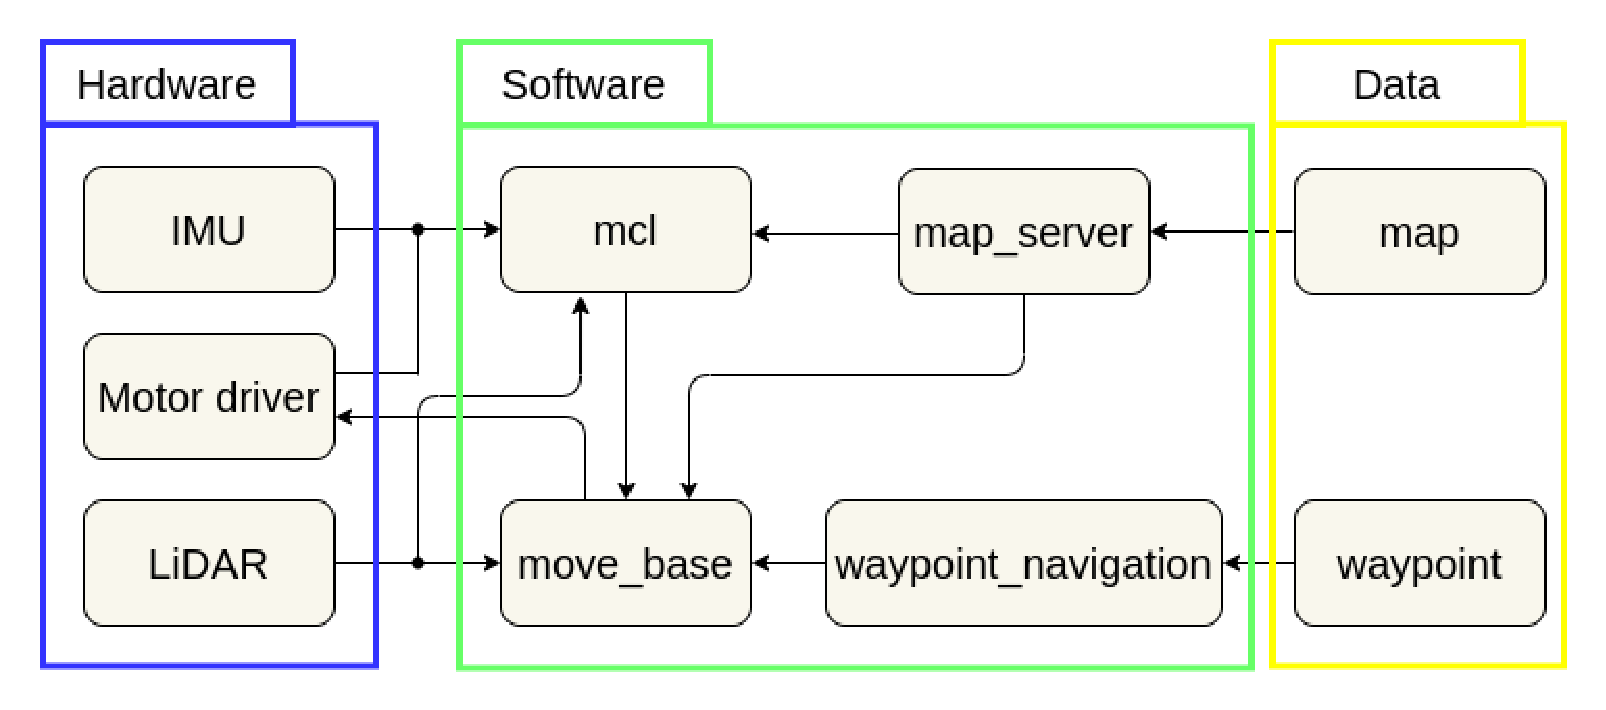
\includegraphics[width=90mm]{fig/software.pdf}
  \caption{Structure of the system.}
  \label{fig:soft-fig}
\end{figure}

\vspace*{2mm}

\section{各ロボットごとの研究開発}
本研究室では,使用するロボットごとに研究開発の目的が異なる.つくばチャレンジ2023においては,
ORNE-box2を使用するチームとORNE-box3を使用するチームの2つに分かれて研究開発を行ってきた.
以降,それぞれのチームをbox2チーム,box3チームと呼ぶこととする.
本章では,各チームごとの取り組みを述べる.

\subsection{box2チームの取り組み}
box2チームは,つくばチャレンジ2022において,記録走行で完走している.しかし,本走行では道路端で
一時停止に失敗し,記録は 320[m]であった.一時停止失敗の原因としては,自己位置推定の破綻が挙げられる.
ORNE-box2では,本走行前日にロボットの制御に使用していたコンピュータである Jetson AGX Xavier が
起動しなくなるトラブルが発生したため,急遽 GIGABYTE GB-BXi7H-4500 に交換を行っていた.
これにより計算処理が間に合わなかったおそれがある.

よって本年度は,基本的には昨年度と同じシステムを用いて完走することを目的とした.
なお,制御用のコンピュータには,記録走行完走時に用いていた Jetson AGX Xavier を使用した.
本年度の取り組みを以下で紹介する.

\subsubsection{センサ・システム構成}
box2チームは,LiDAR,ホイールエンコーダ,IMU,RGBカメラというセンサ構成で実験走行および本走行に臨んだ.
特徴としては,\figref{fig:box2-sensor}のように 2つの LiDAR を用いている点が挙げられる.
上部は自己位置推定用,下部は障害物回避用と使い分けることで,自己位置推定を正確に行いつつ,
低層の障害物などを検出して回避するという狙いがある.ここで,上部に取り付けた LiDAR は,3D-LiDAR であるが,
pointcloud\_to\_laserscan\cite{pointcloud} により,得られた3次元点群を圧縮し,2次元の点群として利用している.
また,ロボットの上部に取り付けたカメラは,選択課題 D1 に取り組む際に使用した.

\begin{figure}[h!]
  \centering
  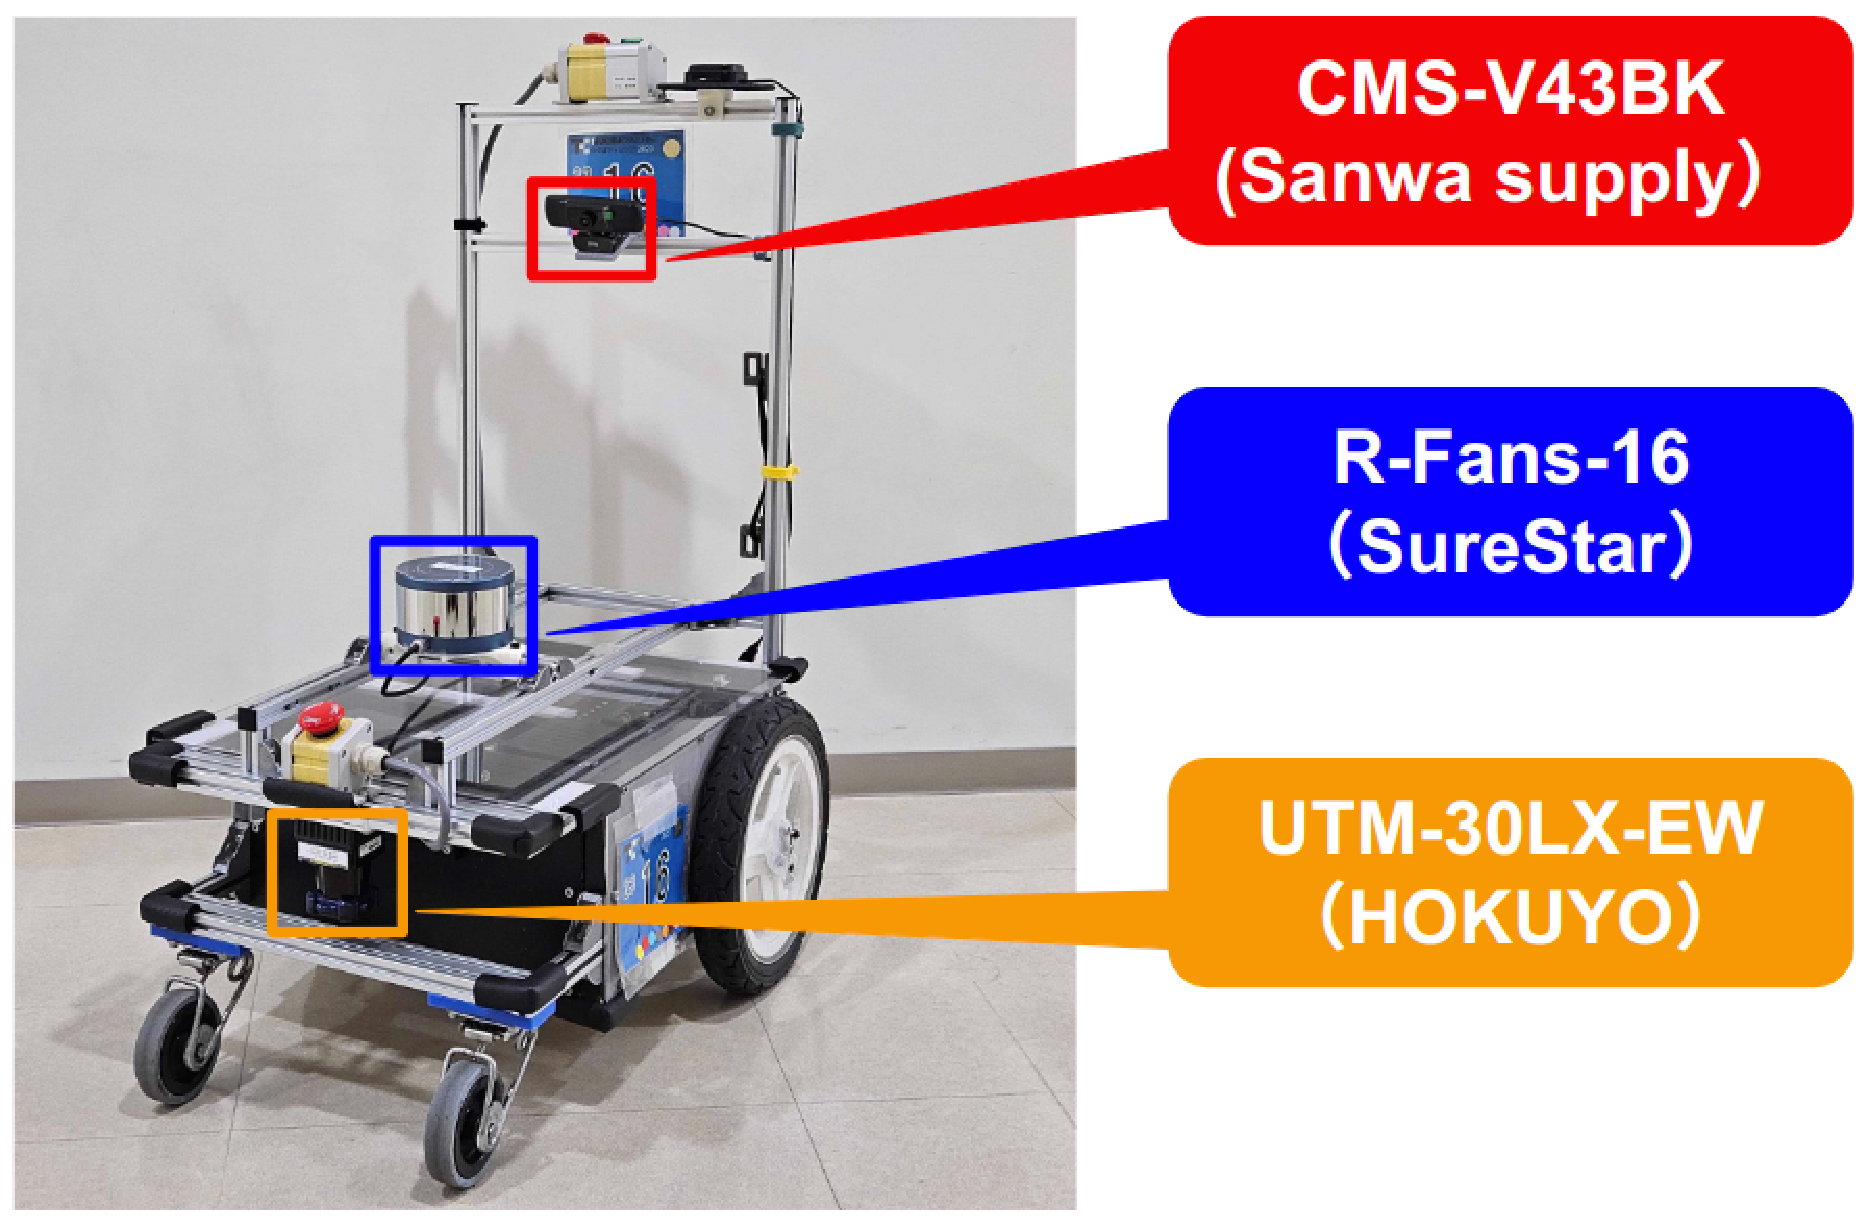
\includegraphics[width=90mm]{fig/box2_sensor_cut2.pdf}
  \caption{The sensor configuration of the box2 team.}
  \label{fig:box2-sensor}
\end{figure}


さらに,自律走行時のシステム構成を以下に示す.

\begin{itemize}
  \item 自己位置推定パッケージ:emcl2\cite{emcl2}
  \item センサ情報統合パッケージ:robot\_localization\cite{robotlocalization}
  \item waypoint パッケージ:waypoint\_manager\cite{waypoint}
  \item global planner:dijkstra
  \item local planner:TrajectoryPlannerROS
  \item map
\end{itemize}


\subsubsection{地図生成}
自律走行時に使用する地図の作成には,Cartographer\cite{Cartographer}を用いた.
ここで,本走行において使用した占有格子地図を\figref{fig:map},\figref{fig:costmap}に示す.
\figref{fig:map}は,自己位置推定に使用する地図であり,基本的には作成時のものから手を加えていない.
\figref{fig:costmap}は,経路計画に用いる地図である.\figref{fig:map}の自己位置推定に用いる地図に
侵入不可能な領域を設定している.これにより,ロボットは侵入不可能領域以外で
経路を生成するようになる.さらに,領域を囲うことで,経路を計算する領域が減るため,
コンピュータの負荷を減らすことができる.
これらの地図は,確認走行エリア,その先から信号あり横断歩道,公園エリアのそれぞれで作成した
地図を合成している.地図の合成や編集には,GIMP\cite{gimp}を用いた.
ちなみに,resolutionは 0.10[m/pixel]で,ファイルのサイズは 17.8 MBであった.

\begin{figure}[h!]
  \centering
  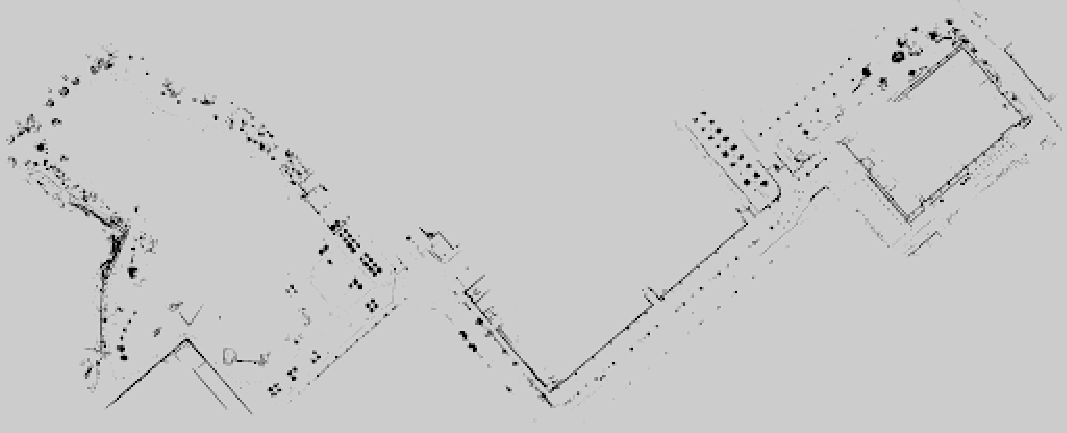
\includegraphics[width=90mm]{fig/map.pdf}
  \caption{Map used for localization.}
  \label{fig:map}
\end{figure}
\vspace*{-1mm}
\begin{figure}[h!]
  \centering
  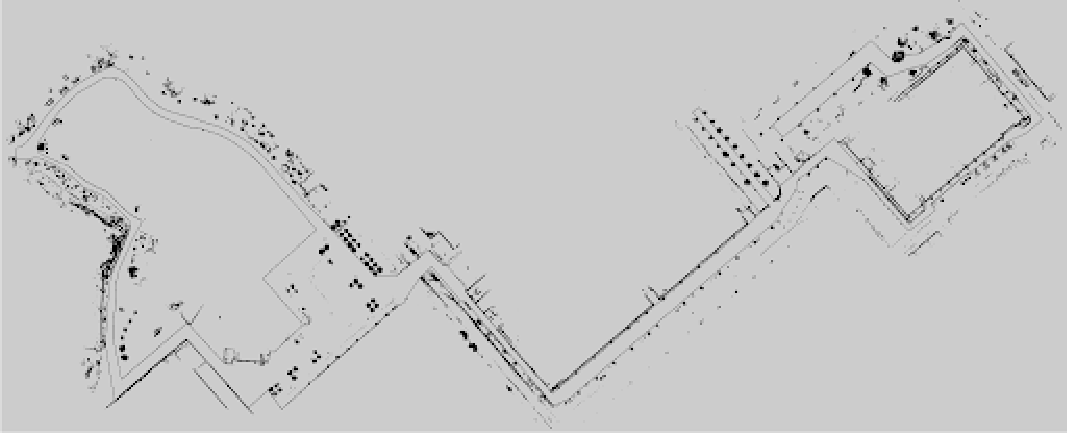
\includegraphics[width=90mm]{fig/costmap.pdf}
  \caption{Map used for planning.}
  \label{fig:costmap}
\end{figure}





% ---------------中村担当(他の部分は変更しないでください)------------------------------
\subsubsection{選択課題 D1}
box2チームでは,本年度から新しく追加された選択課題D1にも取り組んだ.
ここで,課題の概要を述べる.本課題は以下の流れで行う.\\

\hspace*{-1zw}1)集荷ボックス(緑の箱)の待機列に整列\\
2)白線を認識し,その手前 1[m]以内で一時停止\\
3)オペレータ操作により走行再開\\
4)集荷ボックスに50[cm]まで接近し,3秒以上停止\\
5)配達先ラベルを認識後,90秒以内に移動\\
6)指定の宅配ボックス(青)を探索\\
7)指定の宅配ボックスに50[cm]まで接近し,3秒以上停止\\

ここに図貼って説明追加

ただし,検証段階であったため,本走行での使用には至っていない.
% ----------------------------ここまで---------------------------------------------------







\subsubsection{本走行の結果}
box2チームの本年度の本走行の記録は,715[m]であった.
リタイアした地点は,公園前の信号機あり横断歩道である.
\figref{fig:box2-result}に示すように,本来は一時停止が必要な場所で,ロボットが道路端からはみ出した.
原因としては,自己位置推定の破綻が挙げられる.信号機周辺は他チームのロボットや通行人,自動車など,
その都度環境が大きく変化するため,作成した地図とマッチングしない,あるいは誤った場所でマッチング
が起こったのではないかと考えられる.

なお box2チームは,8月18日に実施されたつくばチャレンジ2023EX@イーアスつくば本走行にて完走している.

\begin{figure}[h!]
  \centering
  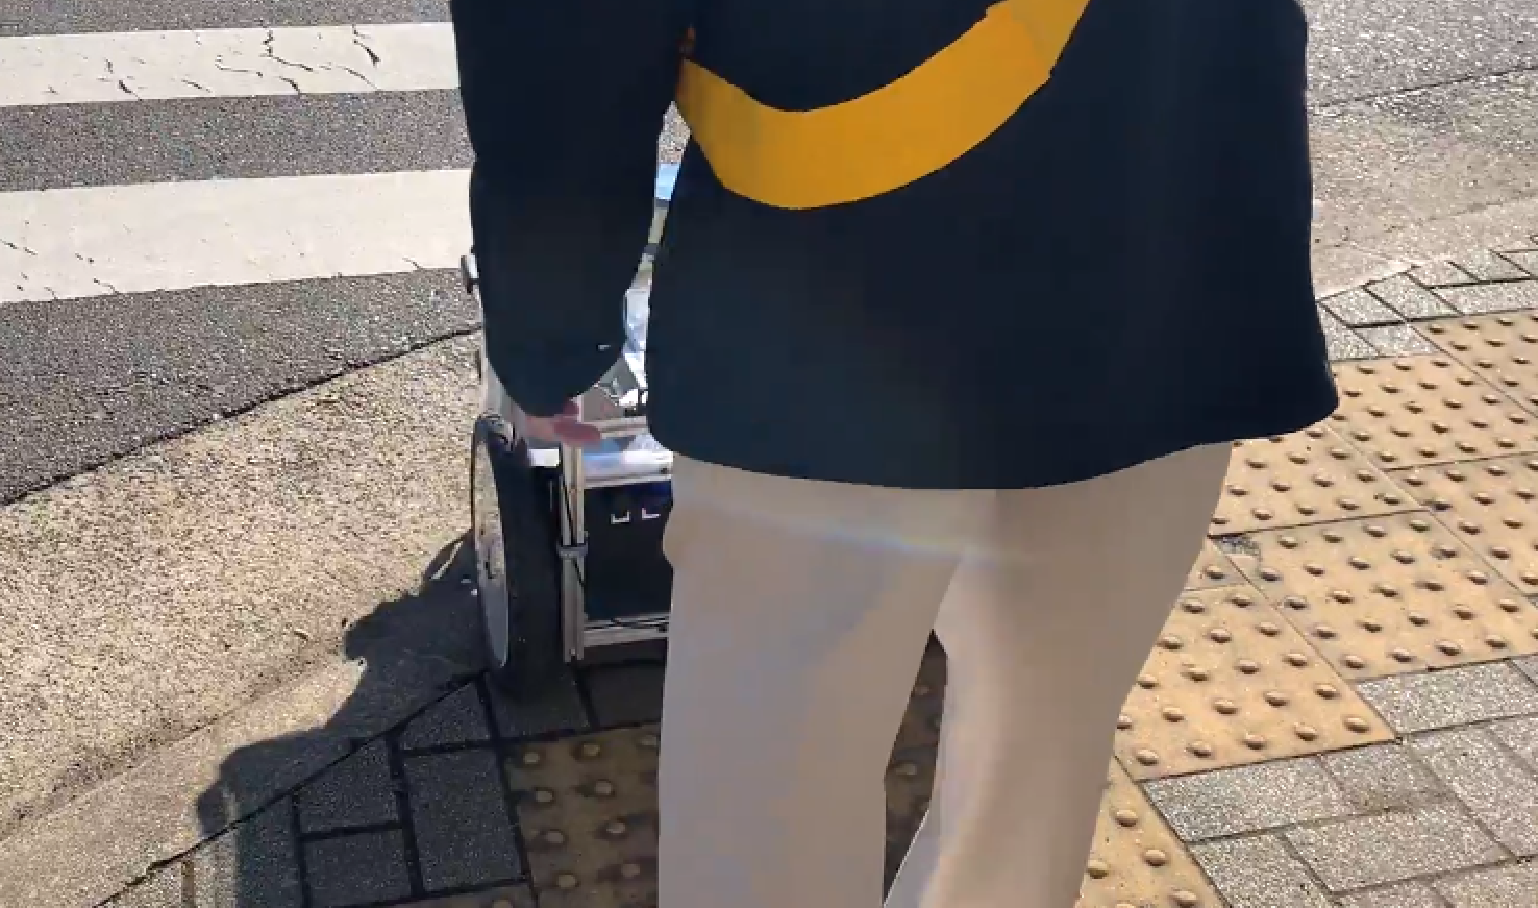
\includegraphics[width=90mm]{fig/result_box2_cut.pdf}
  \caption{box2 team.}
  \label{fig:box2-result}
\end{figure}



\subsection{box3チームの取り組み}
ROS2 Dockerなど、、、
本年度の取り組みを以下で紹介する.

\subsubsection{センサ・システム構成}
box3 チームは,LiDAR,ホイールエンコーダ,RGBカメラというセンサ構成で実験走行および本走行に臨んだ.
box2 チームとは異なり,使用した LiDARは 1つである.
ここで,LiDAR は,3D-LiDAR であるが,
3次元点群を圧縮し,2次元の点群として利用している.
また,ロボットの上部に取り付けたカメラは,信号認識に取り組む際に使用した.

\begin{figure}[h!]
  \centering
  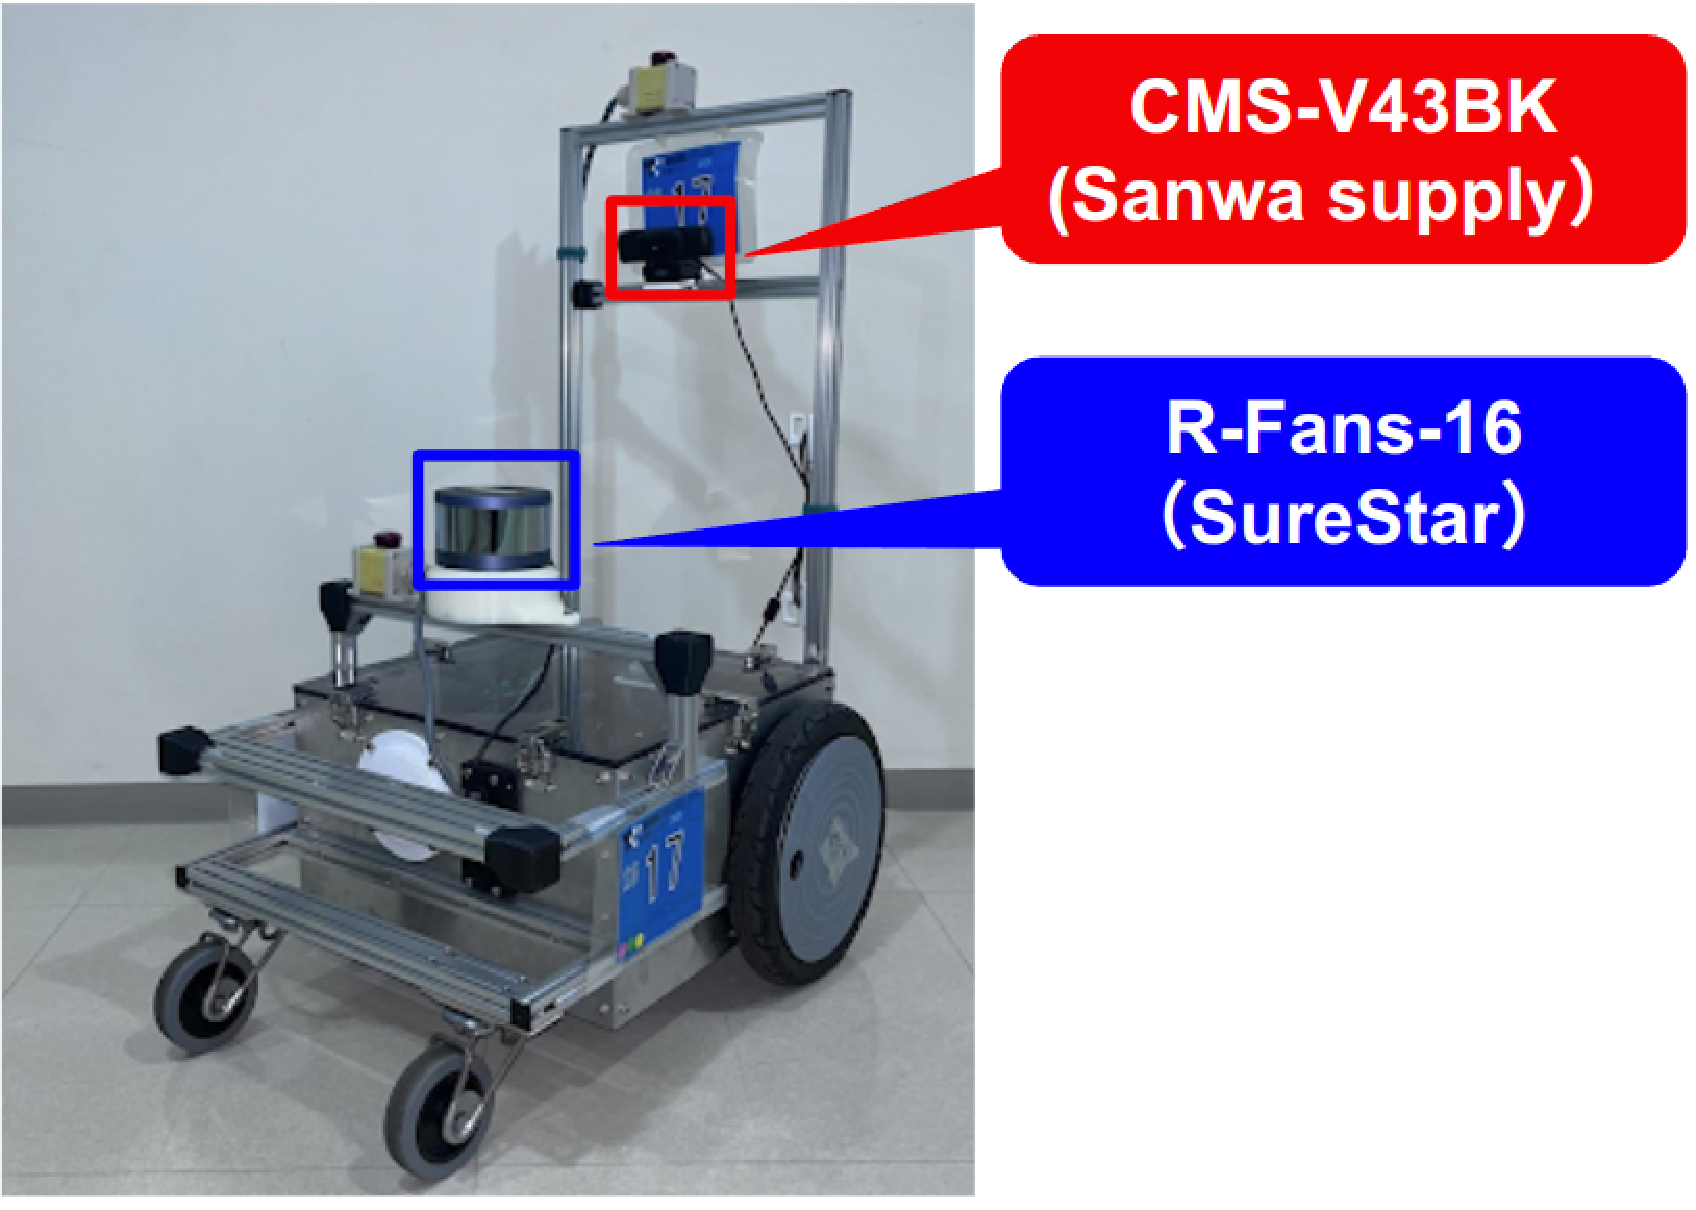
\includegraphics[width=90mm]{fig/box3_sensor.pdf}
  \caption{The sensor configuration of the box3 team.}
  \label{fig:box3-sensor}
\end{figure}


さらに,自律走行時のシステム構成を以下に示す.

\begin{figure}[h!]
  \centering
  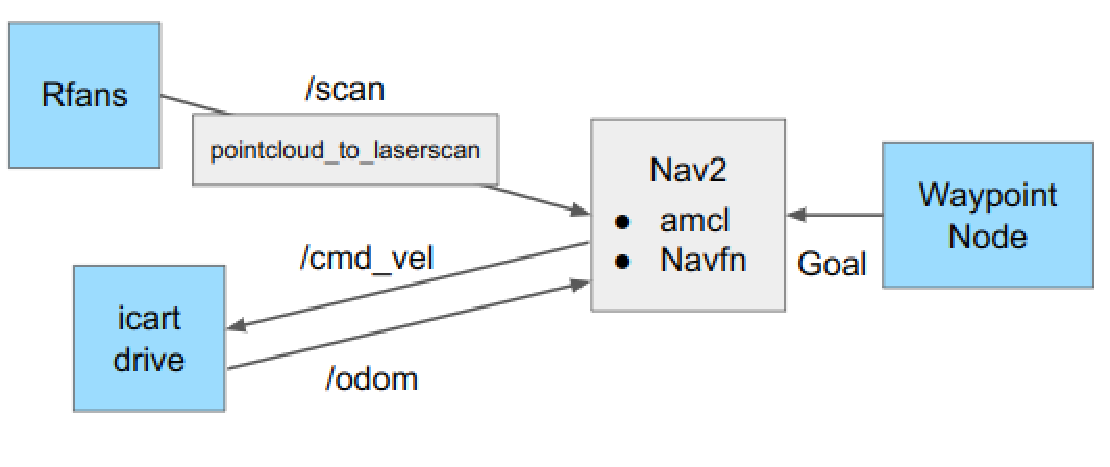
\includegraphics[width=90mm]{fig/box3_system.pdf}
  \caption{The sensor configuration of the box3 team.}
  \label{fig:box3-system}
\end{figure}


\subsubsection{信号認識}
ああああああ

\begin{figure}[h!]
  \begin{minipage}[t]{0.47\linewidth}
    \centering
    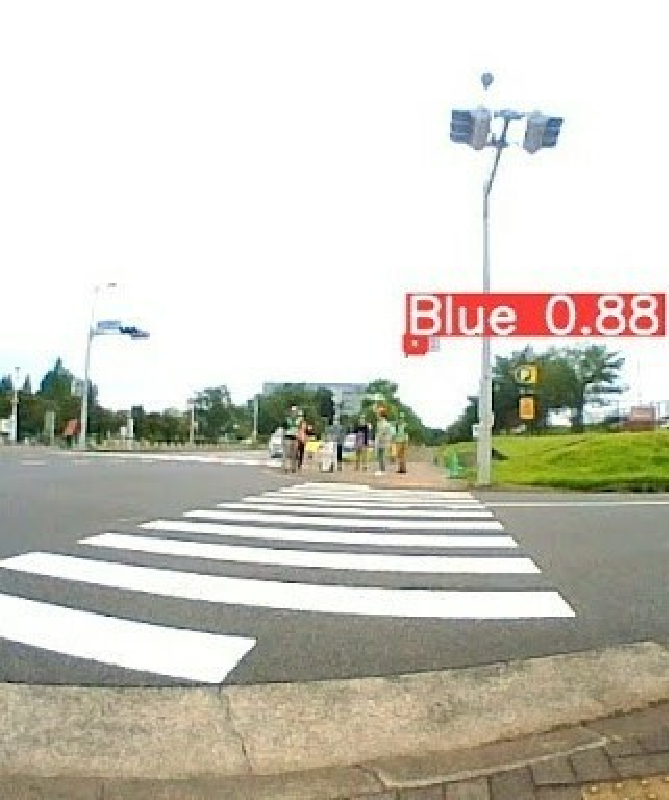
\includegraphics[width=45mm]{fig/blue_cut.pdf}
    \caption*{(a) ORNE-box2}
  \end{minipage}
  \hspace*{2mm}
  \begin{minipage}[t]{0.47\linewidth}
    \centering
    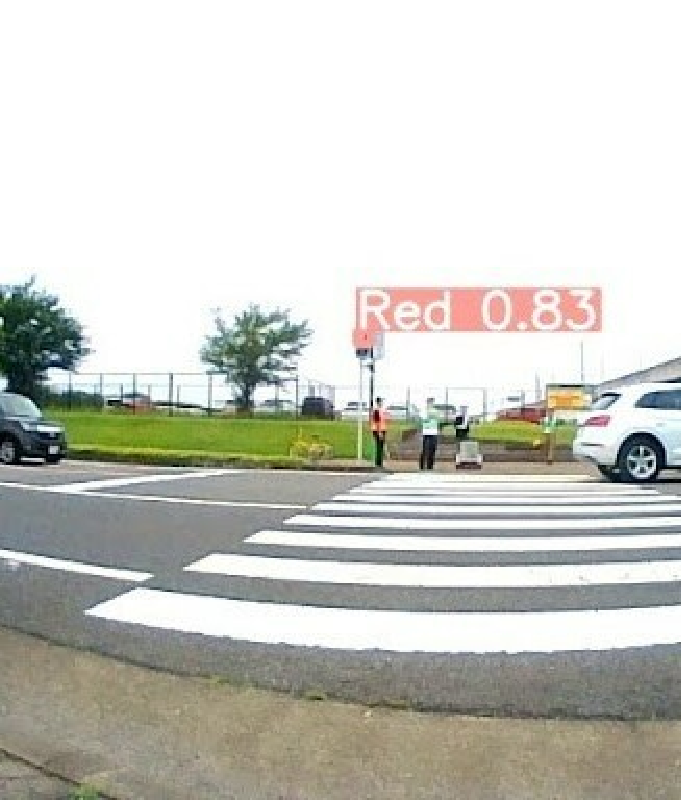
\includegraphics[width=45mm]{fig/red_cut.pdf}
    \caption*{(b) ORNE-box2}
  \end{minipage}%\vspace*{2mm}
  \caption{Number of return to path}
\end{figure}

\subsubsection{本走行の結果}
ああああ
記録走行では431[m]



\section{結言}
本稿では,千葉工業大学未来ロボティクス学科 box2,box3チームで開発しているロボットとシステムの構成に
関して述べた.また,つくばチャレンジ2023に向けた取り組みについて紹介した.\\

\section*{謝辞}
つくばチャレンジ実行委員会の皆様およびつくば市の皆様に感謝申し上げます.また,上田研究室の皆様には
つくばチャレンジ2023の参加にあたり,ご意見やご協力をいただき感謝申し上げます.\\


% 参考文献
% \small
\footnotesize
\begin{thebibliography}{99}

\bibitem{box}
井口 颯人, 石江 義規, 樋高 聖人, 上田 隆一, 林原 靖男 : “ 屋外自律移動ロ
ボットプラットフォーム ORNE-box の開発 ”, 3H2-03 , SI2021(2021)

\bibitem{box-data}
open-rdc, orne-box, wiki\\
\url{https://github.com/open-rdc/orne-box/wiki}\\
(最終閲覧日:\today)

\bibitem{icart}
T-frog Project\\
\url{https://t-frog.com/forums/forum.php?ml=icart-mini-devel}\\
(最終閲覧日:\today)

\bibitem{navigation}
ros-planning, navigation リポジトリ\\
\url{https://github.com/ros-planning/navigation}\\
(最終閲覧日:\today)

\bibitem{orne-navigation}
open-rdc, orne\_navigation リポジトリ\\
\url{https://github.com/open-rdc/orne_navigation}\\
(最終閲覧日:\today)

\bibitem{orne-box}
open-rdc, orne-box リポジトリ\\
\url{https://github.com/open-rdc/orne-box}\\
(最終閲覧日:\today)

\bibitem{open-rdc}
Robot Design and Control Lab, open-rdc, リポジトリ\\
\url{https://github.com/open-rdc}\\
(最終閲覧日:\today)

\bibitem{pointcloud}
ROS wiki, pointcloud\_to\_laserscan\\
\url{https://wiki.ros.org/pointcloud_to_laserscan}\\
(最終閲覧日:\today)

\bibitem{emcl2}
ryuichiueda, emcl2 リポジトリ\\
\url{https://github.com/ryuichiueda/emcl2}\\
(最終閲覧日:\today)

\bibitem{robotlocalization}
cra-ros-pkg, robot\_localization リポジトリ\\
\url{https://github.com/cra-ros-pkg/robot_localization}\\
(最終閲覧日:\today)

\bibitem{waypoint}
masakifujiwara1, waypoint\_manager リポジトリ\\
\url{https://github.com/masakifujiwara1/waypoint_manager}\\
(最終閲覧日:\today)

\bibitem{Cartographer}
cartographer-project, cartographer リポジトリ\\
\url{https://github.com/cartographer-project/cartographer}\\
(最終閲覧日:\today)

\bibitem{gimp}
GIMP 公式ドキュメント\\
\url{https://www.gimp.org/}\\
(最終閲覧日:\today)

\end{thebibliography}
\normalsize

\end{document}
